%\documentclass[aps,preprint,amsmath,amssymb]{revtex4-1}% APS journal style
%\documentclass[aps,reprint,amsmath,amssymb,prl]{revtex4-1}% APS journal style prl physical review letters
\documentclass[aps,reprint,amsmath,amssymb,pra]{revtex4-1}% APS journal pra default
%\documentclass[aps,reprint,amsmath,amssymb,prl,longbibliography]{revtex4-1}% to show the title of the articles in the bibliography
\usepackage{graphicx}% Include figure files
\usepackage{dcolumn}% Align table columns on decimal point
\usepackage{bm}% bold math
\usepackage{hyperref}% add hypertext capabilities
%\usepackage{lineno}
%\linenumbers
%\bibliography{natbib}

\begin{document}
\title{A toy model to understand the dynamics of the vortical motions in turbulent boundary layers}
\author{J.C. Cuevas Bautista}
\email{jcc1@wildcats.unh.edu}
\affiliation{University of New Hampshire, Department of Mechanical Engineering, Durham 03824, USA.}
\date{\today}
\begin{abstract}
\noindent 
Recent studies indicate that the structure of the turbulent boundary layer at high Reynolds number (\textit{Re}) is composed of large uniform momentum zones segregated by fissures of concentrated vorticity. Experiments reveal that the dimensionless fissures thickness (scaled by boundary layer thickness) is $\mathcal{O}(1/\sqrt{Re})$ and the dimensionless streamwise velocity jump across a fissure scales with the friction velocity $\mathcal{O}(u_{\tau})$. A toy model that captures the essential elements of the turbulent boundary layer structure at high \textit{Re} is constructed to evaluate the long-time averaged flow statistics of the boundary layer. First, a ``master'' instantaneous  streamwise velocity profile in the wall-normal direction is constructed by placing a discrete number of fissuress across the boundary layer thickness. The number of fissures and their wall-normal locations follow scalings informed by the Mean Momentum Balance (MMB) theory. Next, the wall-normal positions of the fissures are allowed to randomly move in the wall-normal direction creating a statistically independent second instantaneous velocity profile. This process is then repeated to create an ensemble of instantaneous velocity profiles from which average statistics of the turbulent boundary layer can be computed and assessed. The statistics of the toy model are compared to statistics acquired in turbulent boundary layers at high \textit{Re}.
\end{abstract}
\keywords{turbulent boundary layer, uniform momentum zones, vortical fissures and Mean Momentum Balance theory.}
\maketitle
\section{\label{sec:intro} Introduction}
Turbulent boundary layer and its mechanism is one the most active research area in fluid mechanics. Due to its chaotic behaviour, deterministic approaches are not possible. However there is a general consensus in the scientific community about that turbulent boundary layers exhibit similar statistical properties. One of the stronger hypothesis  support the idea that the smoothness in the average of the streamwise velocity profile is caused by the spatial average of multiple instantaneous velocity profiles with different zones of uniform momentum~\citep{mca1995,umz2015}. In this article a toy model is attempted to demonstrate this assertion.\\
The mean streamwise velocity profile is reproduced by average different instantaneous velocity profiles with a different distribution of uniform momentum zones.
The phenomenological description of the structure of the uniform momentum zones through the boundary layer has been studied by several authors~\citep{nose}. They suggest that UMZ are the result of the interaction of the wider range of structures that populate the turbulent boundary layer\cite{2} such as hairpins and streamwise vortices. \cite{amt2000} Adrian, Meinhart and Tomkins have made a thoroughly  study about how the vortex structures are organized and segregate the UMZs in turbulent boundary layers.  These studies indicate that theses regions of uniform momentum are segregated by smaller structures named vortical fissures.\citep{priya2007} Priyadarshana does a good description of what a vortical fissure looks like and how they can be distributed in the mean velocity profile (see Fig.~\ref{fig:vortical_fissures}). 
\begin{figure}[b]
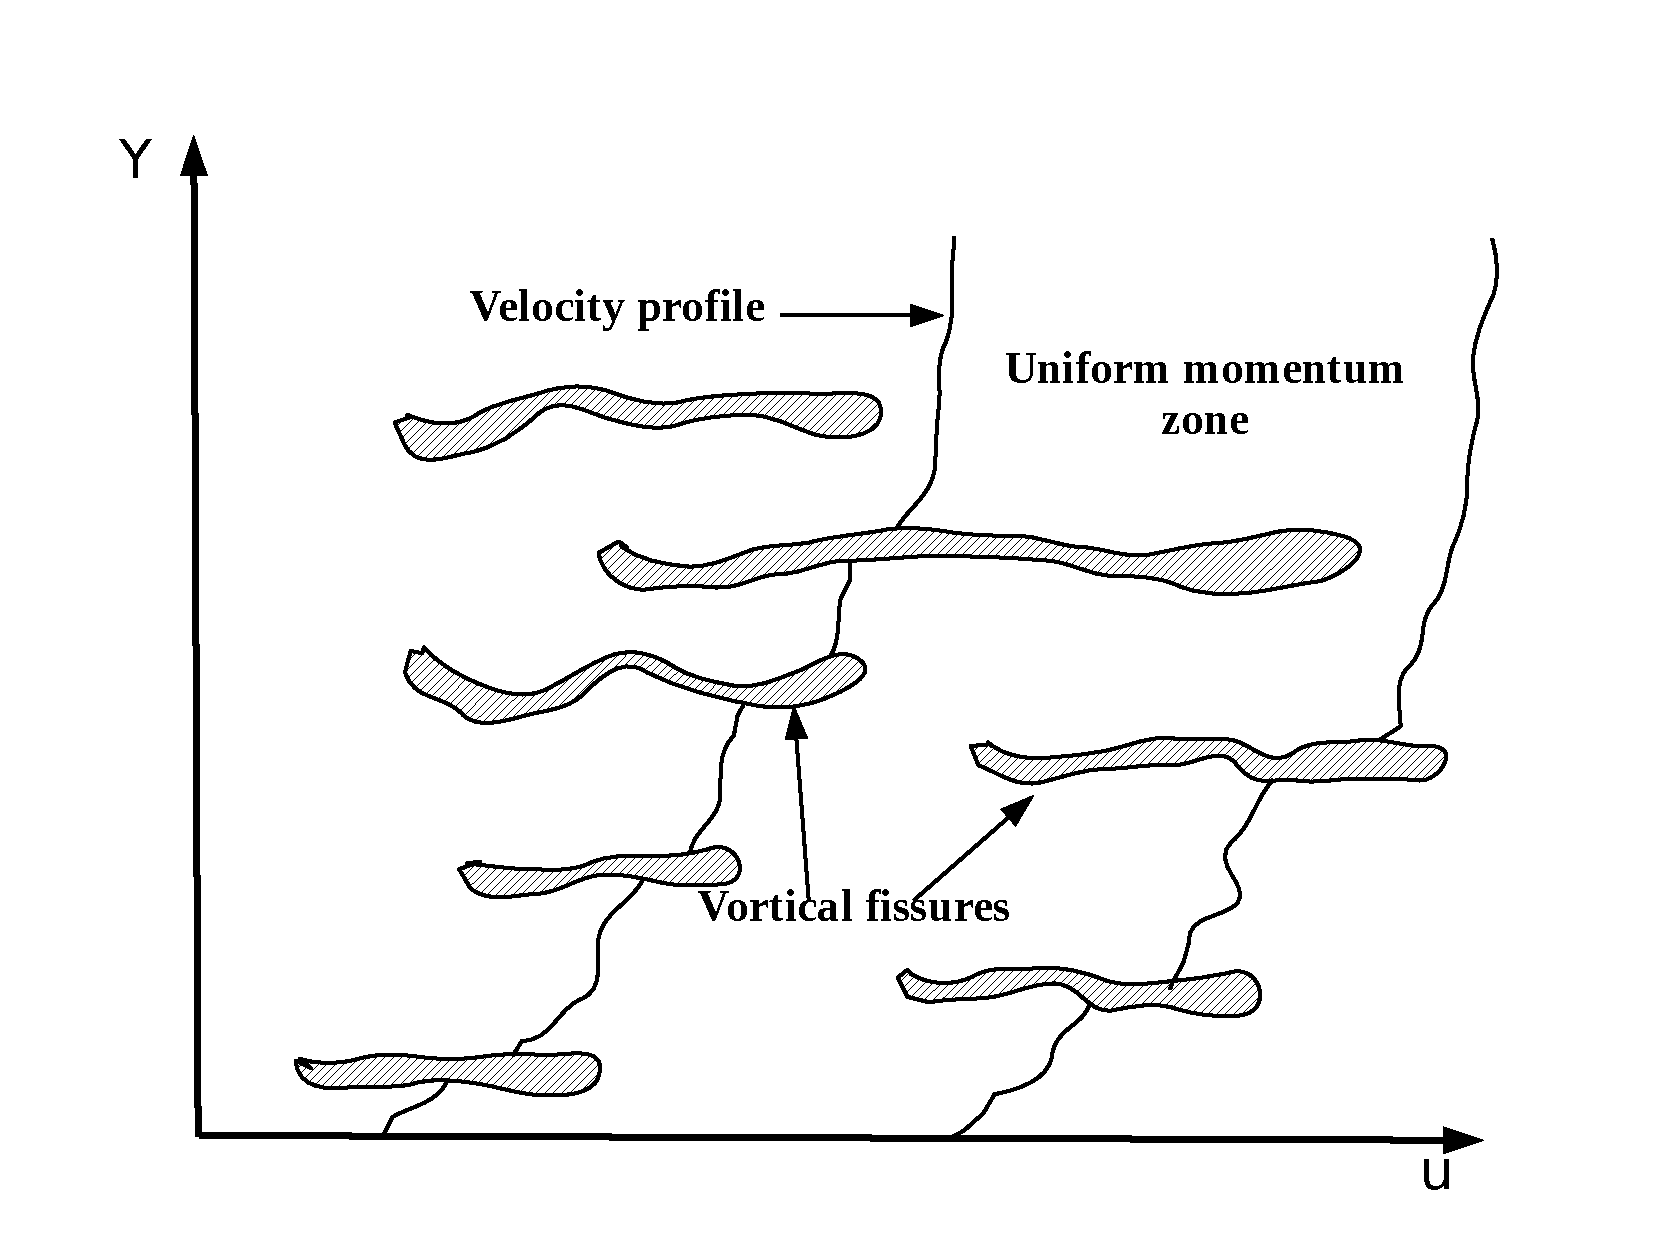
\includegraphics[scale=0.33]{figures/uniform_velocity_vortical_fissures}
\caption{\label{fig:vortical_fissures} Pictorial representation of instantaneous velocity profiles like zones of uniform momentum separated by zones of concentrated vorticity (vortical fissures).
Adapted from~\citep{priya2007}}
\end{figure} 
Where $U$ is the mean velocity in the x direction (streamwise) and $y$ is the wall normal coordinate.
He explains that the vortical fissures are regions of concentrated vorticity where viscous effects are significative. Vortical fissures can be also a representation of a more complex 3d structures, i.e they can be seen like the transversal section of a hairpin vortex in the streamwise-wall-normal plane \cite{amt2000}. This zonal arrangement could explain somehow the traditional structure of layers in the mean velocity profile for a turbulent boundary layer. Namely the viscous, subwoofer, logarithmic and outer layer in  the classical theory\citep{tenelumley}. The physics of the turbulent boundary layers is embedded in the Navier-Stokes Equations (NSE), as we know they still lack of a closure relationship. Classical theory has successfully found closed solutions to NSE by use asymptotic and multiple scales methods. However a new model seem to describe more accurately the dynamics of turbulent flows according with the mean momentum equation. Klewicki~\citep{Klewickimmb} describes correctly how the Mean Momentum Balance theory predict the physical characteristics for canonical flows as well as the classical theory does. Some of the properties of the scaling for the four-layer structure in the mean streamwise velocity profile are summarized in Table~\ref{tab:4layerstructure},

\begin{table}[htb]%
\caption{\label{tab:4layerstructure}%
Scaling associated to the four layer structure from MMB theory. $\Delta y$ represents the thickness of the layer while $\Delta u$ is the velocity increment associated to that layer in the turbulent boundary layer.
}
\begin{ruledtabular}
\begin{tabular}{ccc}
\textrm{Layer}&
\textrm{$\Delta y$}&
\textrm{$\Delta u$}\\
\colrule
I &$\mathcal{O}(\nu/u_{\tau})(\lesssim 3)$&$\mathcal{O}(u_{\tau})(\lesssim 3)$\\
II &$\mathcal{O}(\sqrt{\nu\delta/u_{\tau}})(\sim 1.6)$&$\mathcal{O}(U_{\infty})(\sim 0.5)$\\
III &$\mathcal{O}(\sqrt{\nu\delta/u_{\tau}})(\sim 1.0)$&$\mathcal{O}(u_{\tau})(\sim 1)$\\
IV &$\mathcal{O}(\delta)(\rightarrow 3)$&$\mathcal{O}(U_{\infty})(\rightarrow 0.5)$ \\
\end{tabular}
\end{ruledtabular}
\end{table}
The length and velocity scales has been normalized by the viscous units $\nu$ and $u_{\tau}$, where $u_{\tau}=\sqrt{\tau_{\omega}/\rho}$ is the friction velocity, $\tau$ is the mean wall shear stress and $\nu$ is the kinematic viscosity. Likewise the outer units $\delta$, the boundary layer thickness and $U_{\infty}$ the free-stream velocity. Layer I can be seen like the equivalent to the viscous sublayer in the conventional theory, layer II is the stress gradient balance layer, layer III  is denominated mesolayer where all the forces in the MME balances and layer IV which makes reference to the inertial layer or logarithmic layer since inertial effects are dominant. In the toy model proposed here we attempt to describe and predict the behaviour of the inertial layer. Various models have attempted to reproduce the dynamics of turbulent boundary layers using different structures like hairpin structures~\citep{adrian2007} or eddy structures~\citep{perry1995}, however there is not a reference at least to the knowledge of the author where the statistics of turbulent boundary layers are reproduced by used the MMB theory along with the uniform momentum zones concept. In fact the previous models are somehow dynamical models in the sense that they are the result either of numerical simulations (DNS) or they combines momentum equation assumptions with self-similarity restrictions (eddy geometries). The model proposed here is a phenomenological model in the sense that there are not dynamical equations to solve or specific geometries involved, it is rather an observational model where a little of reverse engineering is applied.\\

In this paper we present a simplified toy model to reproduce the higher order moments of the streamwise turbulent boundary layers. Likewise the model is tuned up in such way that we are able to verify if this uniform-momentum zonal structure average creates an inertial region by examine the indicator function $\beta$~\cite{}. DNS data for a channel flow at friction Reynolds number $\delta^+=\delta u_{\tau}/\nu\approx 5200$ ~\cite{leemoser2015}  along with scaling reported by MMB theory was used to build the model. 

\section{\label{sec:nm} Numerical Methods}
A  mean step master stream-wise velocity profile is represented within the boundary layer by a set of $N$ discrete velocity steps spaced according to  
\begin{align}
U^+_{i+1}=&U^+_i+\phi_c^2 ln(\phi_c) \label{eq:upvel},\\
y^+_{i+1}=&\phi_c y^+_i\quad i=0,\ldots ,N-1. \label{eq:yppos}
\end{align}
Where expressions~\eqref{eq:upvel} and~\eqref{eq:yppos} are derived from the MMB theory~\citep{Klewickimmb}.~\eqref{eq:upvel} determines the increments in the stream-wise normalized velocity $U^+$, the width of the steps in the $x$ coordinate while~\eqref{eq:yppos} determines the increments in the normalized wall normal position $y^+$, the height of the steps in the y coordinate (See Fig.~\ref{fig:master_profile}). The golden ratio $\phi_c$ is given by $\phi_c=(1+\sqrt{5})/2$~\cite{klewicki2014} and the thickness of the
vortical fissures $\mathcal{O}(1/\sqrt{Re})$ is considered negligible at high $Re$. For the lower boundary conditions was assumed that $y^+_0=\phi_c\sqrt{\delta^+}$ in order to coincide with the onset of the logarithmic region  while $U^+_0=0.5 U_{\infty}^+$ to be the half of the normalized free-stream velocity $U_{\infty}^+$ (see table~\ref{tab:4layerstructure}). \\  
The upper boundary conditions are defined in such way that the last position $y_{N}^+$ of the vortical fissure and its associated velocity $U^+_{N}$ is constrained by $y_{N}^+\approx\delta^+$.\\
\begin{figure}[b]
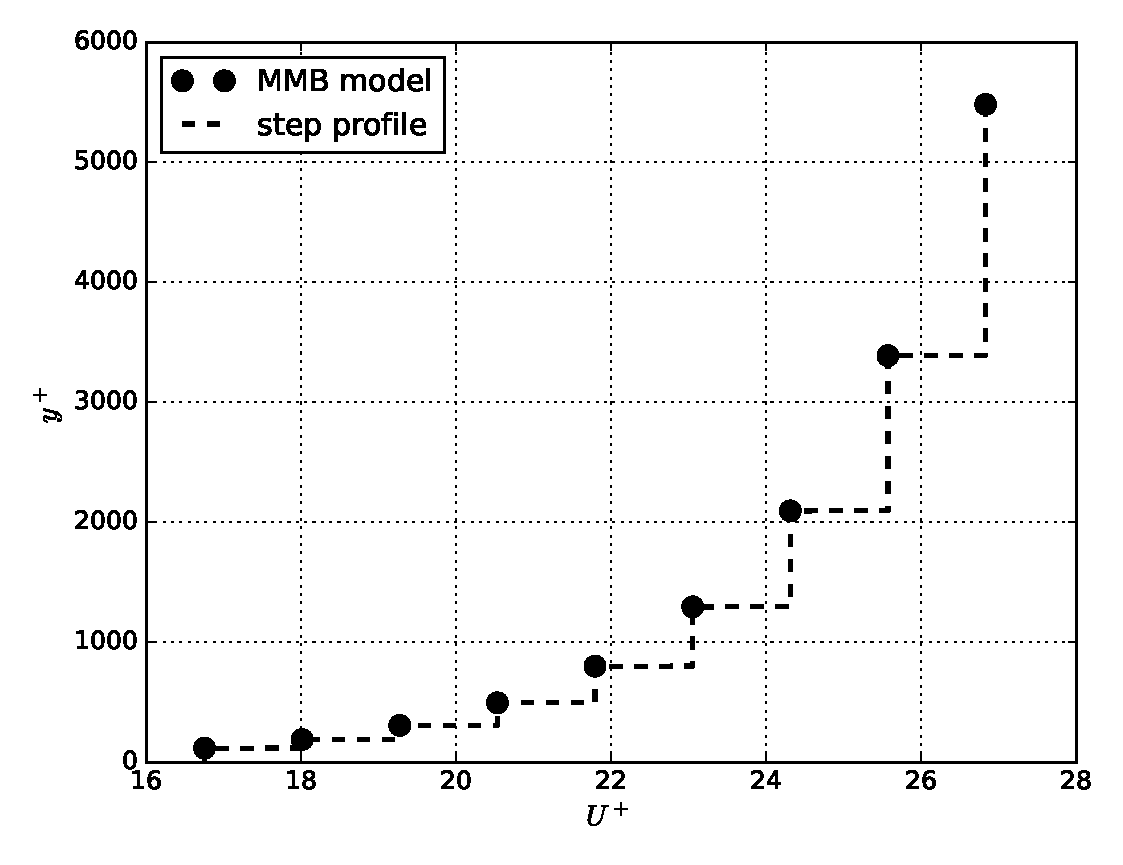
\includegraphics[scale=0.46]{figures/Master_step_profile}
\caption{\label{fig:master_profile} Mean step velocity master profile (red dashed lines) overlapped with an instantaneous perturbed velocity profile (blue solid line) and the original data points computed by Eqs.~\eqref{eq:upvel} and~\eqref{eq:yppos}. $\delta^+=5200$ and $U^+_{\infty}=26.5$ are from channel DNS~\citep{leemoser2015}.}
\end{figure} 
Fig.~\ref{fig:master_profile} depicts a representative mean step master velocity profile with a grid of $5481$ linearly spaced positions in the wall normal direction each one with an associated streamwise velocity. The dot circles are the velocities and positions of the vortical fissures computed using~\eqref{eq:upvel} and~\eqref{eq:yppos} respectively. Then the zones of uniform momentum are created allocating the velocity of the current vortical fissure to the grid points between the previous and the current vortical fissure. This velocity remains characteristic for each vortical fissure, thus we wave $N-1$ uniform momentum zones, where $N$ is number of the vortical fissures. Note that at higher $\delta^+$ the number of UMZs increases.\\
Next, instantaneous velocity profiles are created by the repositioning of the vortical structures trough the wall normal direction. This is accomplished by add a Gaussian perturbation $GP$ of the actual height $\Delta h^+_i=y^+_i-y^+_{i-1}$ of the uniform momentum zone to the current position of the vortical fissure $y^+_i$, i.e, 
\begin{equation}\label{eq:ypert}
y^+_{new}=y^+_i\pm \Delta h^+_i GP.
\end{equation}
Here we remark that just the position of the vortical fissures are being perturbed though the velocities remains attached to each vortical fissure. Thus zones of higher momentum can reside closer to the wall if the upper vortical fissures move enough downward in the boundary layer. Once the new positions have been computed, we proceed to fill the grid points similarly to the master profile. Fig.~\ref{fig:master_profile} shows how the seventh and eight vortical fissures have moved upwards and the second and third have move downwards respect to their original positions (blue solid line).  Fig.~\ref{fig:mul_profiles} shows five instantaneous velocity step profiles,  it can be seen how the upper vortical fissures resides now in the vicinity of the wall and some lower vortical fissures have moved to intermediate positions, this mechanism allow us to create zones of negative vorticity since the  uniform momentum zones are not increasing monotonically. 
\begin{figure}[b]
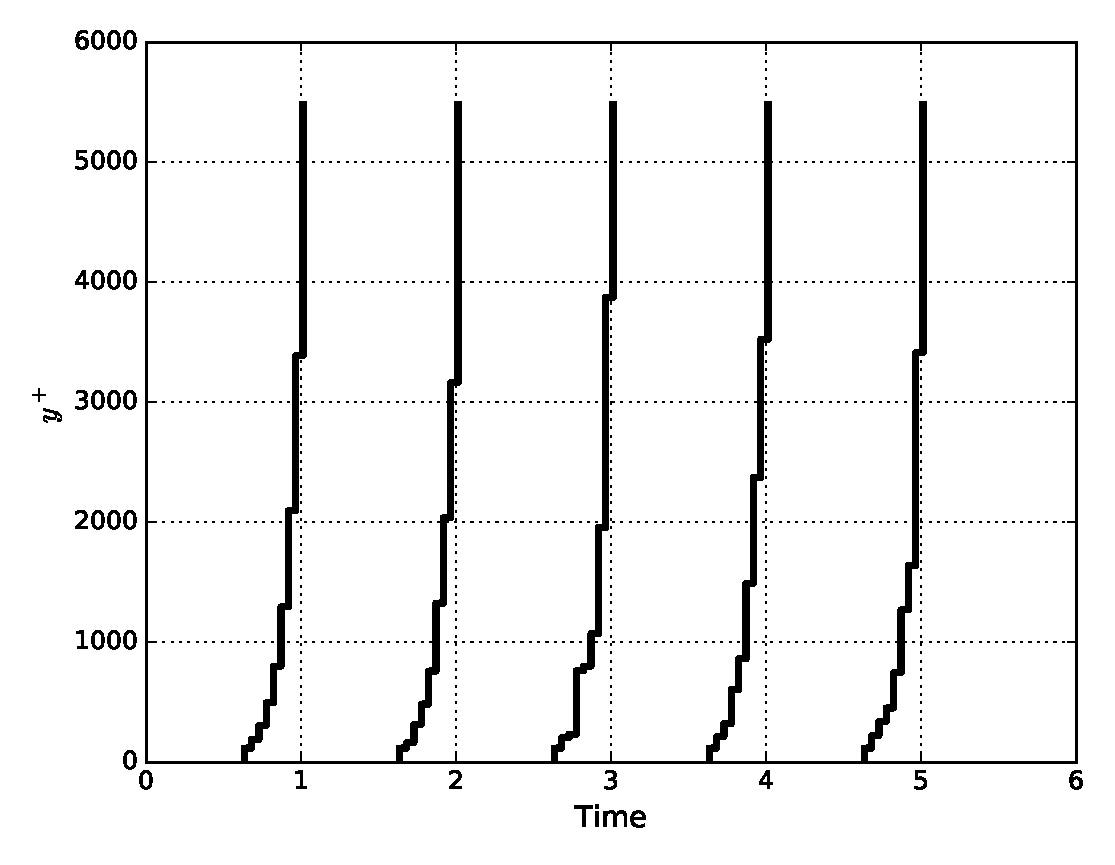
\includegraphics[scale=0.46]{figures/multiple_instantaneous_vprof}
\caption{\label{fig:mul_profiles} Multiple instantaneous velocity profiles with a gaussian perturbation of mean $\mu=0$ and standard deviation $\sigma=0.4$.}
\end{figure}
The multiple instantaneous step velocity profiles are considered independent events since they are the result of the Gaussian perturbation in the wall normal positions of the master profile. Thus to achieve statistical convergence the mean step master velocity profile is constructed by average over 5000 independent realizations.
\section{Mean turbulence statistics analysis}
For the purpose of validate the toy model, the high order moments such as the mean, variance, skewness and kurtosis of the mean turbulent streamwise velocity profile were computed. As described in Sec.~\ref{sec:nm}, not only a Gaussian perturbation was used to randomize the positions of the vortical fissure but also an uniform distribution. These variations attempts to explore if there is a dependence between the perturbation distribution and the statistics of the toy model. Thus a strong agreement between the numerical results either for any perturbation and the experimental data could give us some insight about the statistical nature of this process in a real turbulent flow.
\subsection{Gaussian perturbation}
Multiple scenarios with different standard deviations were investigated for the Gaussian perturbation, however just two are presented here. They represent poor $\sigma=0.4$ and good $\sigma=1$ agreement with the experimental results~\cite{Vincenti2013,FLM}, both with $\mu=0$. First scenario considers that the random variation in the position of the vortical fissures ranges between $-120\%$ and $120\%$ of their current positions, where $3\sigma$ events are less likely to occur. Fig.~\ref{fig:mean_profile} is the turbulent mean velocity profile for $\sigma=0.4$. It can be appreciated regions of relative uniform velocity along with small velocity jumps located close to the unperturbed wall normal positions of the vortical fissures (see Fig.~\ref{fig:master_profile}). These oscillations are similar to the peak-locking phenomena in experimental data, and they are the result of  the velocity average of vortical fissures with identical velocities in the same wall normal positions. Also note that an uniform momentum zone arise from $y^+=0$ to $y^+=118$, these are the velocity boundary conditions imposed in the first position of the vortical fissure which are held fixed. Despite of these discrepancies, the mean velocity profile shows an acceptable agreement with the shape of the experimental data.\\
\begin{figure}[b]
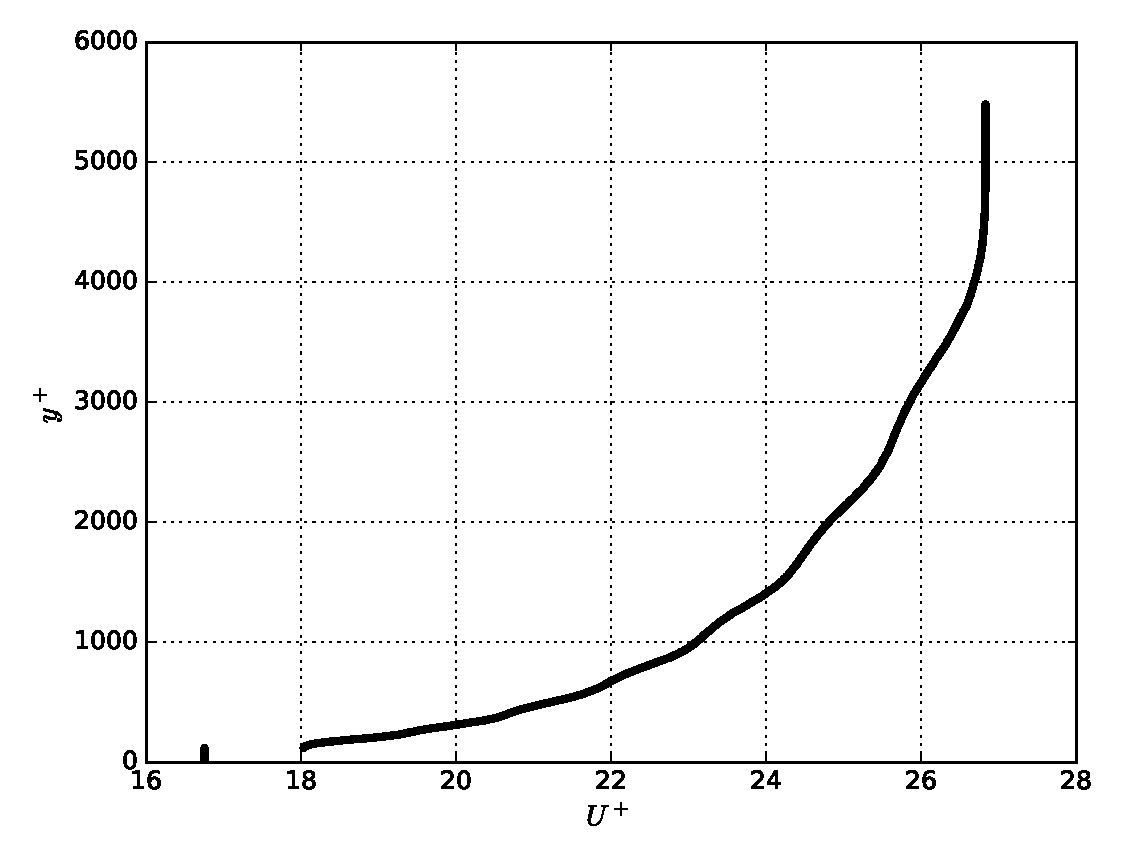
\includegraphics[scale=0.46]{figures/Master_averaged_step_profile_5000_assembles}
\caption{\label{fig:mean_profile} Mean stream-wise velocity profile for 5000 independent realizations with a Gaussian perturbation of $\mu=0$ and $\sigma=0.4$.}
\end{figure}

Fig.~\ref{fig:varigaus} shows the variance of the streamwise fluctuations for $5000$ independent realizations as a function of the wall normal position. Here the peak-locking phenomena is more evident and it could be associated to the use of pseudo-random number generators (PRNG). Since the Gaussian random numbers are not totally independent but they are computed through a deterministic algorithm, wall normal positions can be populated with the same vortical fissures several times~\cite{nm}. It is also remarkable that for this scenario crossing vortical fissures are rarely observed since the random perturbation does not exceed $130\%$ units of their current wall normal positions. 

\begin{figure}[b]
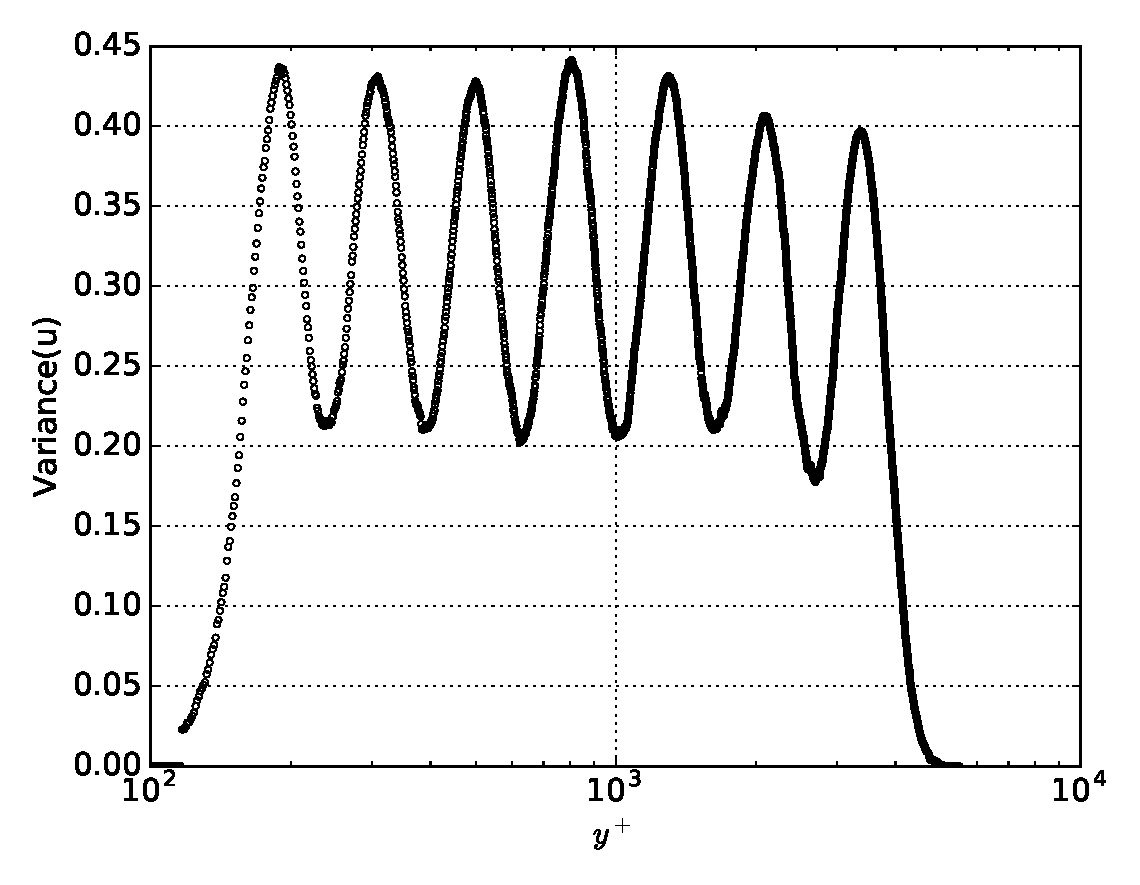
\includegraphics[scale=0.46]{figures/variance_5000_assembles}
\caption{\label{fig:varigaus} Stream-wise velocity variance for 5000 independent realizations with a Gaussian perturbation of $\mu=0$ and $\sigma=0.4$.}
\end{figure}
As is usual Fig.~\ref{fig:skewgaus} shows the skewness for the streamwise fluctuations as a function of the wall normal position on a semi-logarithmic axes plot. The graph shows the correct trend in the lower and the upper edge of the inertial region (Layer III table), i.e. it is maximum in the proximity of the wall and then it reaches its maximum negative value close to the boundary layer thickness $y^+=\delta^+$. However through the inertial region the skewness oscillates with an small amplitude $\pm 1$ around the value for a Gaussian distribution, in contrast with the experimental data that shows a plateau tendency right below of the Gaussian trend. The abrupt variations in the skewness can be also a side effect of peak-locking. Unlike the skewness, the oscillations for the stream-wise velocity kurtosis (Fig.~\ref{fig:kurt}) have a higher amplitude trough the inertial region where the experimental data exhibit an uniform subgaussian trend. This behaviour does not reproduce properly the turbulence statistics and thus we explore higher values of $\sigma$ in the Gaussian perturbation.\\

\begin{figure}[tb]
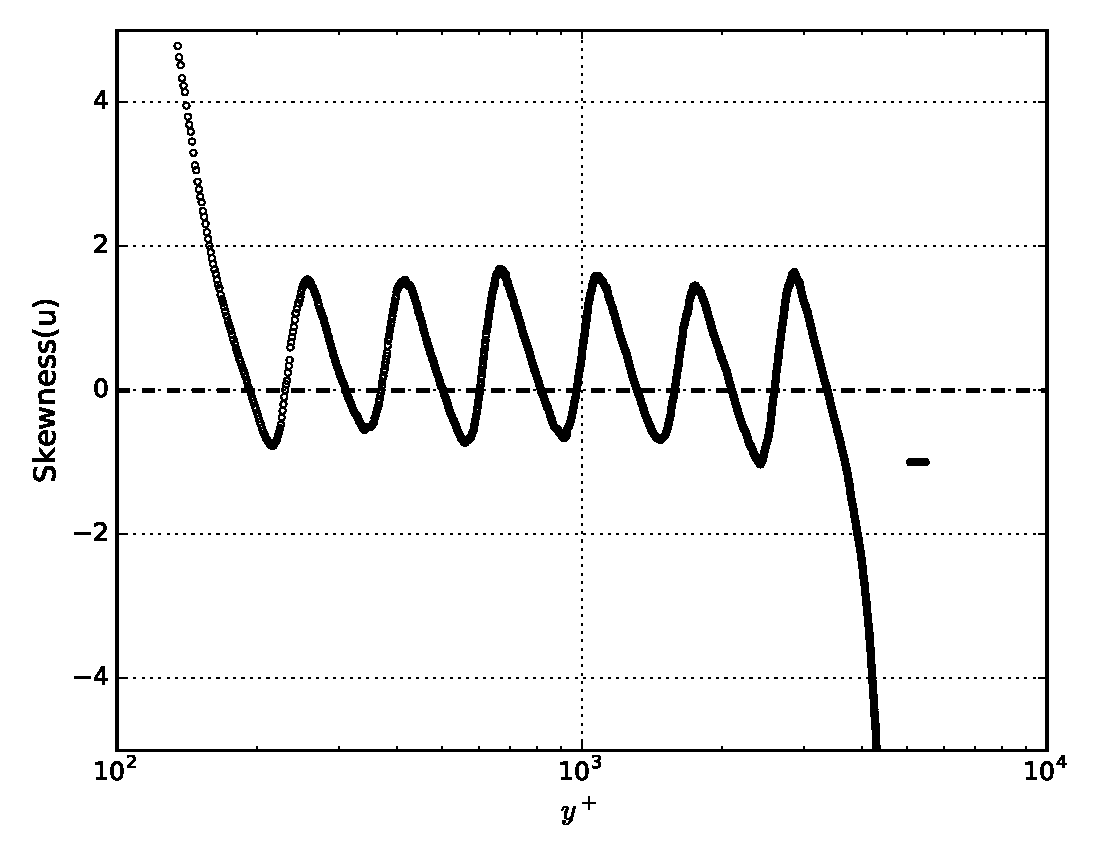
\includegraphics[scale=0.46]{figures/skewness_5000_assembles}
\caption{\label{fig:skewgaus} Skewness of streamwise velocity fluctuations for 5000 independent realizations with a Gaussian perturbation of $\mu=0$ and $\sigma=0.4$ (open circles). The skewness for a Gaussian distribution is plotted in dotted lines as reference.}
\end{figure}
In the second scenario $\sigma=1$ is selected in order to achieve a more homogeneous velocity distribution. This perturbation creates a random vertical motion of the vortical fissures between $-300\%$ and $300\%$ of their respective step height (see Sec.~\ref{sec:nm}). Consequently the vortical fissures in the upper edge of the inertial region can cross and reside close to the wall. The opposite is also true for vortical motions that lie in the onset of the inertial region. Fig.~\ref{fig:mp_gau100} shows a smoother profile compared with $\sigma=0.4$ where peak-locking effect was still present. This mean velocity profile exhibits a good agreement for $\delta^+=5200$ respect to the experimental data. 
\begin{figure}[tb]
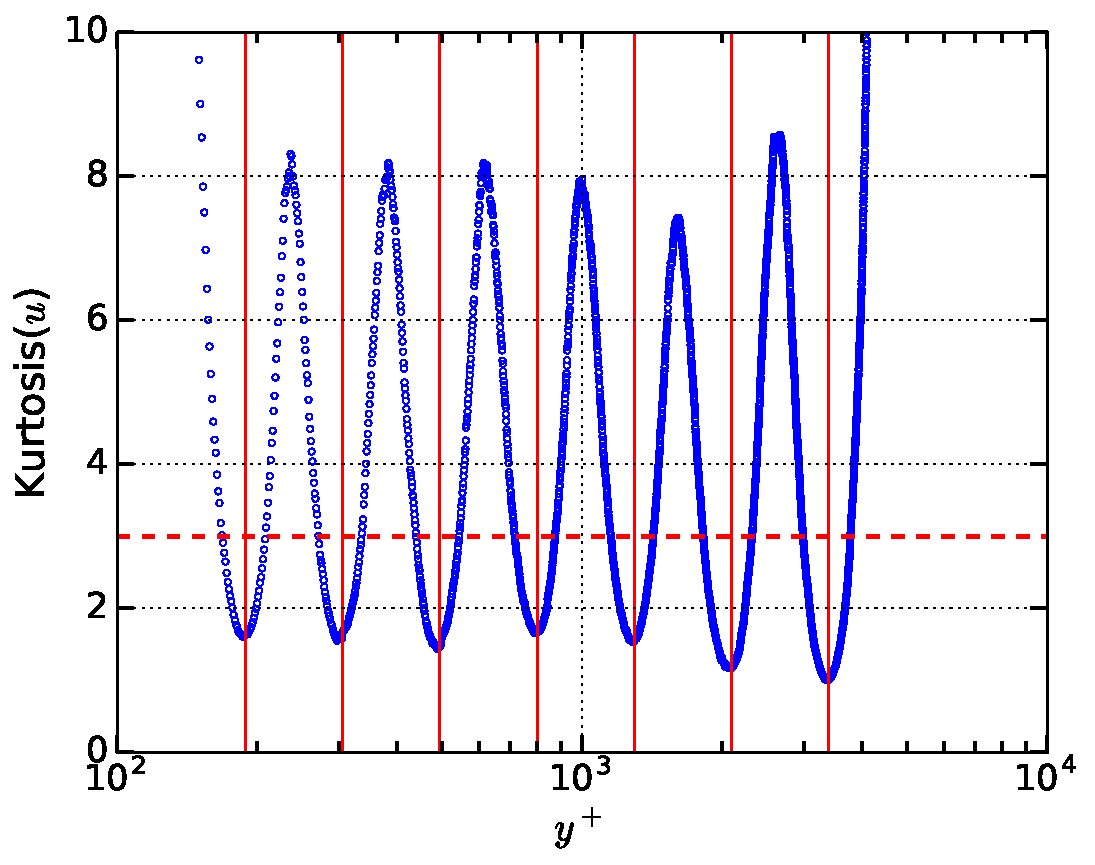
\includegraphics[scale=0.46]{figures/kurtosis_5000_assembles}
\caption{\label{fig:kurt} Kurtosis of streamwise velocity fluctuations for 5000 independent realizations with a Gaussian perturbation of $\mu=0$ and $\sigma=0.4$ (open circles). The kurtosis for a Gaussian distribution is plotted in dotted lines as reference.}
\end{figure}
In addition to the mean, the second, third and fourth order moments are also computed for this scenario. Fig.~\ref{fig:varigaus100} reveals some of the main properties of the stream-wise velocity variance for turbulent flows.  These are the variance is zero in the vicinity of the wall with its maximum value in the onset of the logarithmic region and then decreases almost logarithmically toward the boundary layer edge $y^+=\delta^+$. 
\begin{figure}[tb]
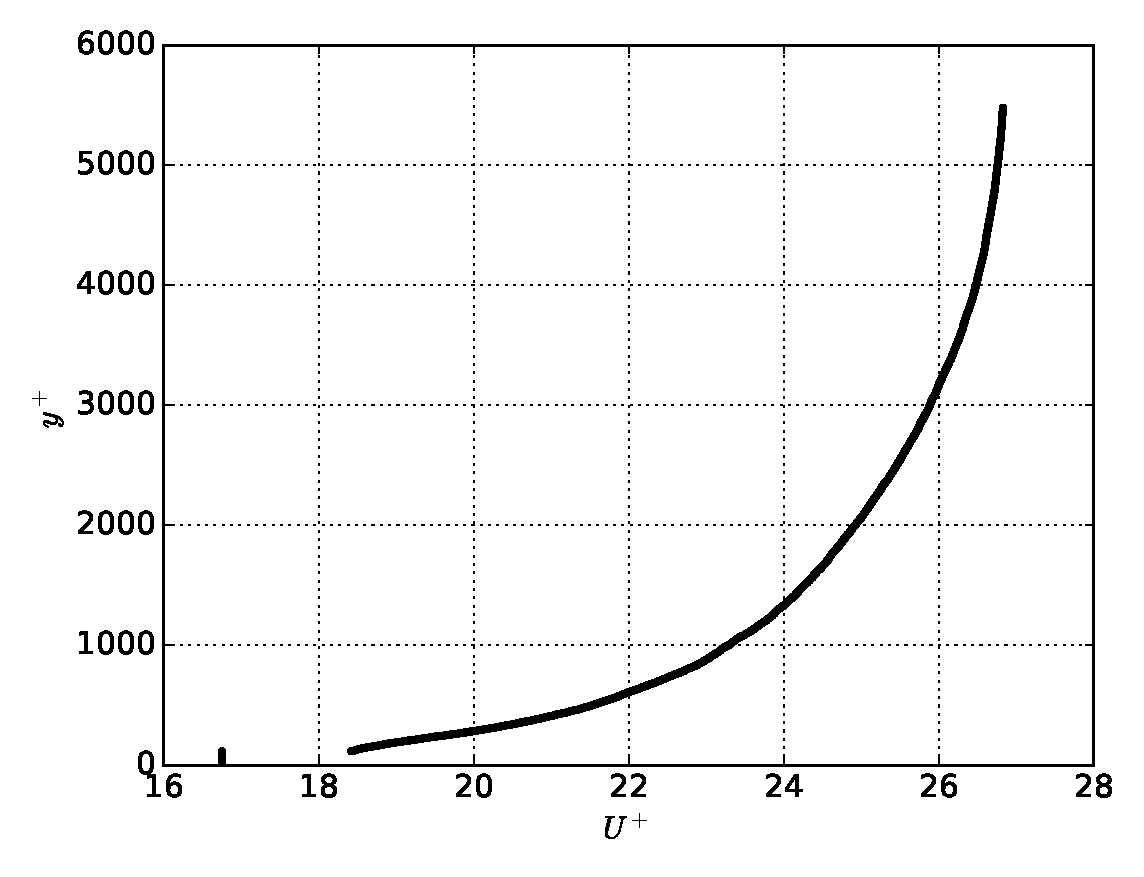
\includegraphics[scale=0.46]{figures/Master_averaged_step_profile_5000_assembles_gaus100}
\caption{\label{fig:mp_gau100} Mean turbulent stream-wise velocity profile for 5000 independent realizations with a Gaussian perturbation of $\mu=0$ and $\sigma=1$.}
\end{figure}
Although the variance is not totally smooth, it is a good improvement over the variance for the first scenario. Also note there is not evidence of peak-locking effect like can be visualized in the third and fourth moments (Figs.~\ref{fig:skewgaus100} and~\ref{fig:kurtgaus100}). 
\begin{figure}[b]
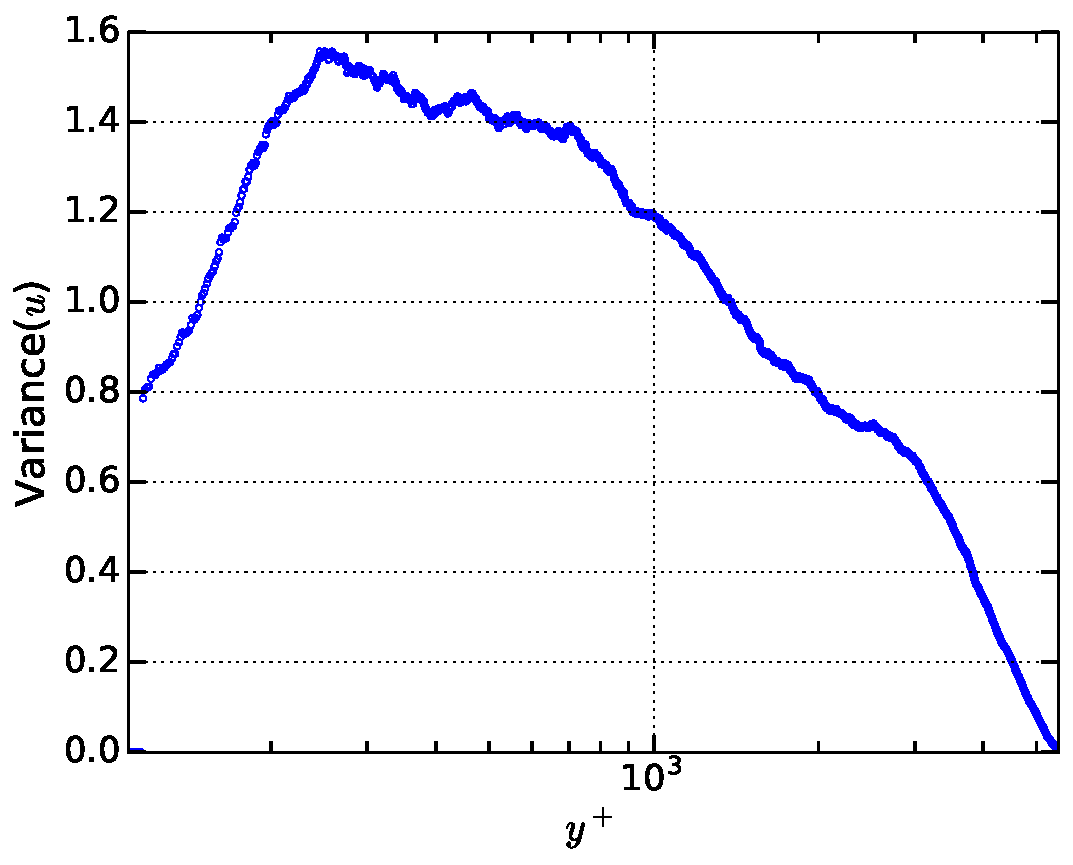
\includegraphics[scale=0.46]{figures/variance_5000_assembles_gauss100}
\caption{\label{fig:varigaus100} Stream-wise velocity variance for 5000 independent realizations with a Gaussian perturbation of $\mu=0$ and $\sigma=1$.}
\end{figure}
Fig.~\ref{fig:skewgaus100} shows the skewness for $\sigma=1$, it can be appreciated how the skewness has its maximum positive value close to the wall and then when it is approaching to the log region exhibits a subgaussian trend that rapidly decays to its maximum negative peak at the end of the logarithmic region. Unlike the experimental results, the boundaries of the skewness in the toy model still do not show the adequate trend. This is caused mainly because the first and last step vortical positions in the model are not being perturbed. Further investigation is necessary to establish the proper boundary conditions in order to improve the agreement near to the wall and away from it in the boundary layer for the turbulent statistics.
\begin{figure}[tb]
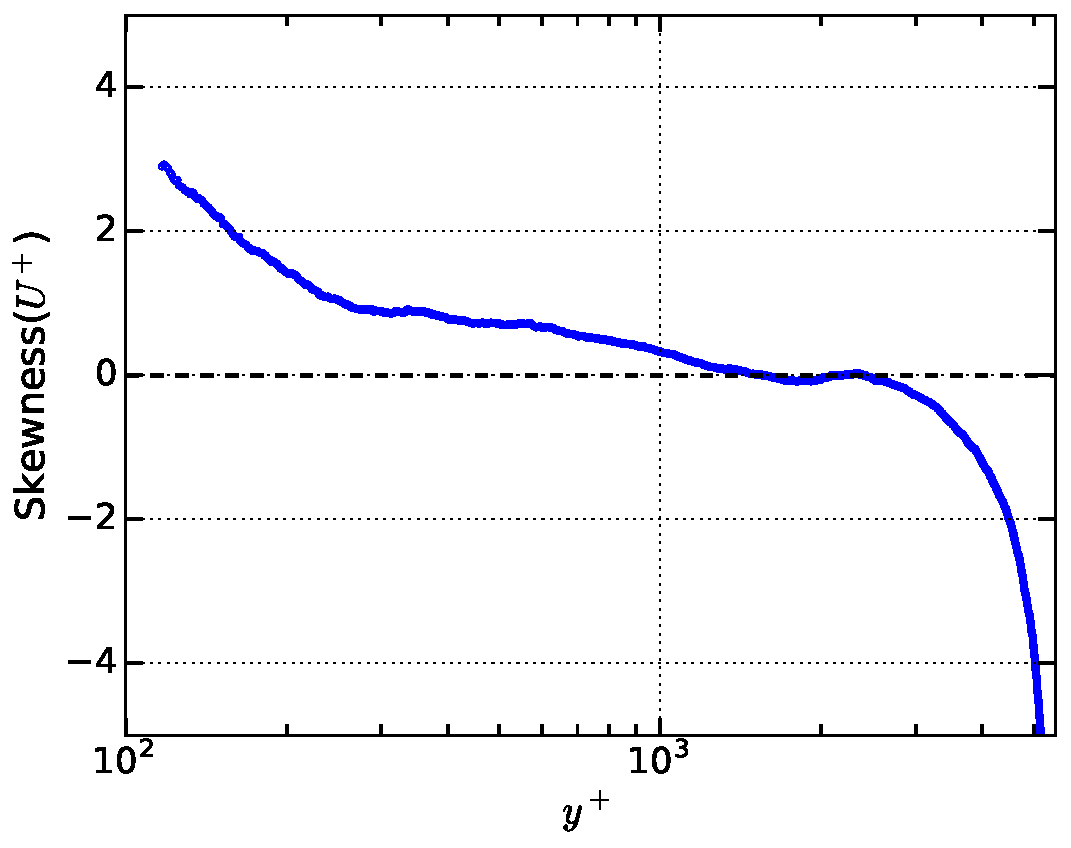
\includegraphics[scale=0.46]{figures/skewness_5000_assembles_gauss100}
\caption{\label{fig:skewgaus100} Skewness of streamwise velocity fluctuations for 5000 independent realizations with a Gaussian perturbation of $\mu=0$ and $\sigma=1$ (open circles). The skewness for a Gaussian distribution is plotted in dotted lines as reference.}
\end{figure}
Observation of Fig.~\ref{fig:kurtgaus100} evidences a similar pattern for the streamwise kurtosis, where the behaviour of the trend in the boundaries does not reproduce the experimental results faithfully. Despite of these discrepancies the kurtosis is very well behaved in the inertial region where it exhibits a subgaussian trend just as the real data do. Experimentally it is expected that the kurtosis reach its maximum value at $y^+=\delta^+$ and then decay in the free-stream region outside to the boundary layer. This is not observed in our results due to the boundary conditions explained previously. However a new distribution to perturb the position of the vortical fissures is attempted, one whose edges decays smoother than the gaussian distribution, thus a dependence on the perturbation distribution can be discarded.
\begin{figure}[tb] 
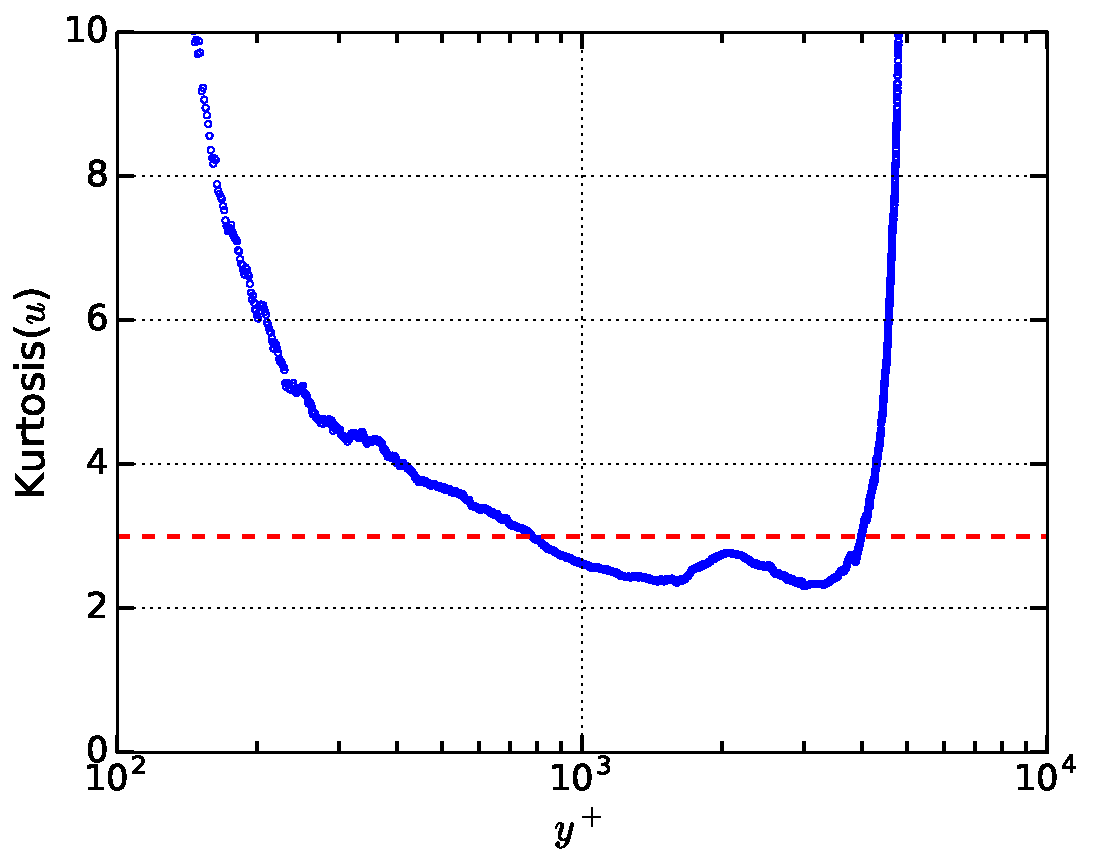
\includegraphics[scale=0.46]{figures/kurtosis_5000_assembles_gauss100}
\caption{\label{fig:kurtgaus100} Kurtosis of streamwise velocity fluctuations for 5000 independent realizations with a Gaussian perturbation of $\mu=0$ and $\sigma=1$ (open circles). The kurtosis for a Gaussian distribution is plotted in dotted lines as a reference.}
\end{figure}
Next section describe the numerical results of the turbulence statistics using an uniform distribution.
\subsection{Uniform distribution}
Previous section suggest that the vortical fissure crossing enhances the creation of a more homogeneous velocity distribution in the boundary layer, therefore an uniform distribution between $-130\%$ and $130\%$ of the height of the step has been selected. Fig.~\ref{fig:mp_un130}  shows the streamwise velocity profile for the uniform perturbation. In comparison with Fig~\ref{fig:mean_profile}, the jumps in the velocity profile seems to have a more straight slope. Since for an uniform distribution, all the vortical positions have the same probability to occur, regions of concentrated velocity such like in the gaussian distribution are not observed. Instead zones with an increasing uniform velocity are appreciated.   
\begin{figure}[htb]
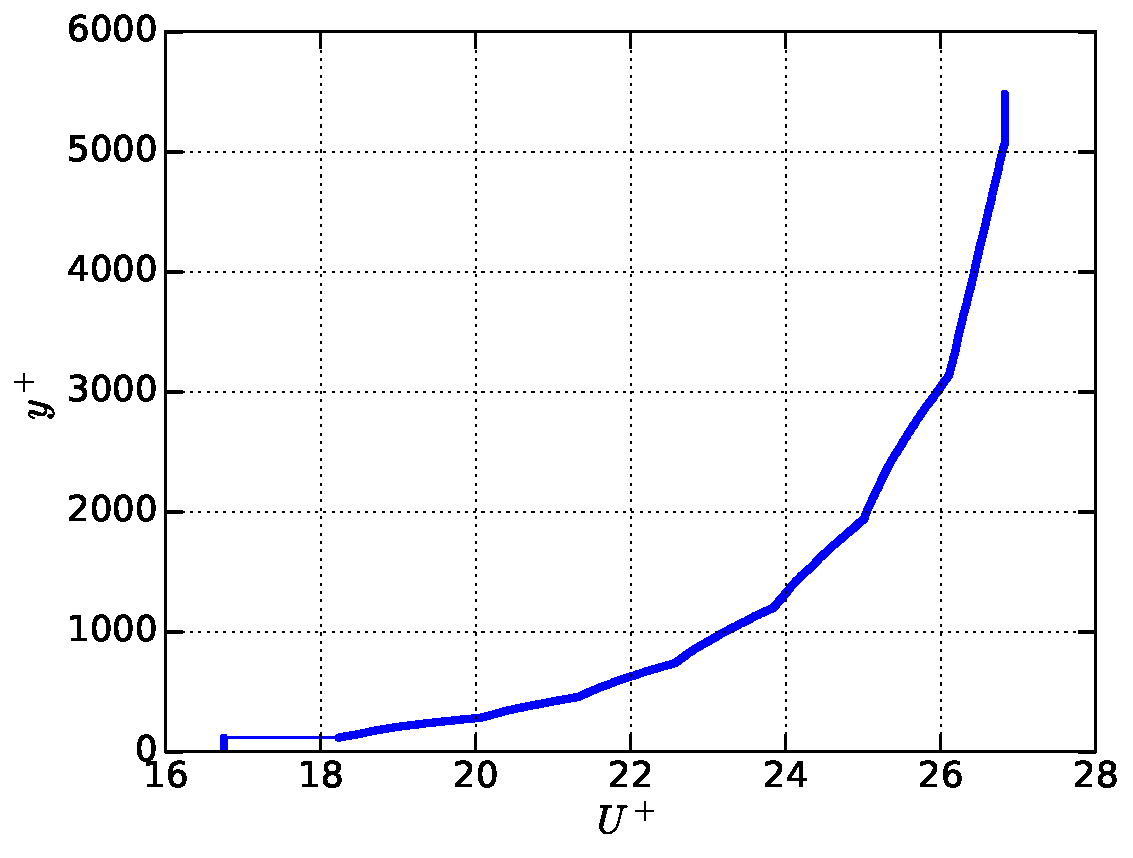
\includegraphics[scale=0.46]{figures/Master_averaged_step_profile_5000_assembles_un130}
\caption{\label{fig:mp_un130} Mean turbulent stream-wise velocity profile for 5000 independent realizations with an uniform perturbation of $\pm 130\%$.}
\end{figure}
This effect can be appreciated more clearly in the stream-wise velocity variance (Fig.~\ref{fig:varun130}), where the variance oscillates around the positions of the vortical fissures in the master profile. These oscillations are characterized by having a smaller amplitude ($\sim 0.2$ units) compared with the Gaussian perturbation for $\sigma=0.4$ (Fig.~\ref{fig:varigaus}). Despite of the oscillations, the main features of the turbulence variance are conserved. For instance it has a peak in the proximity of the wall and then a pronounced negative slope in the inertial region up to reach zero in the upper edge of the inertial region.\\
\begin{figure}[htb]
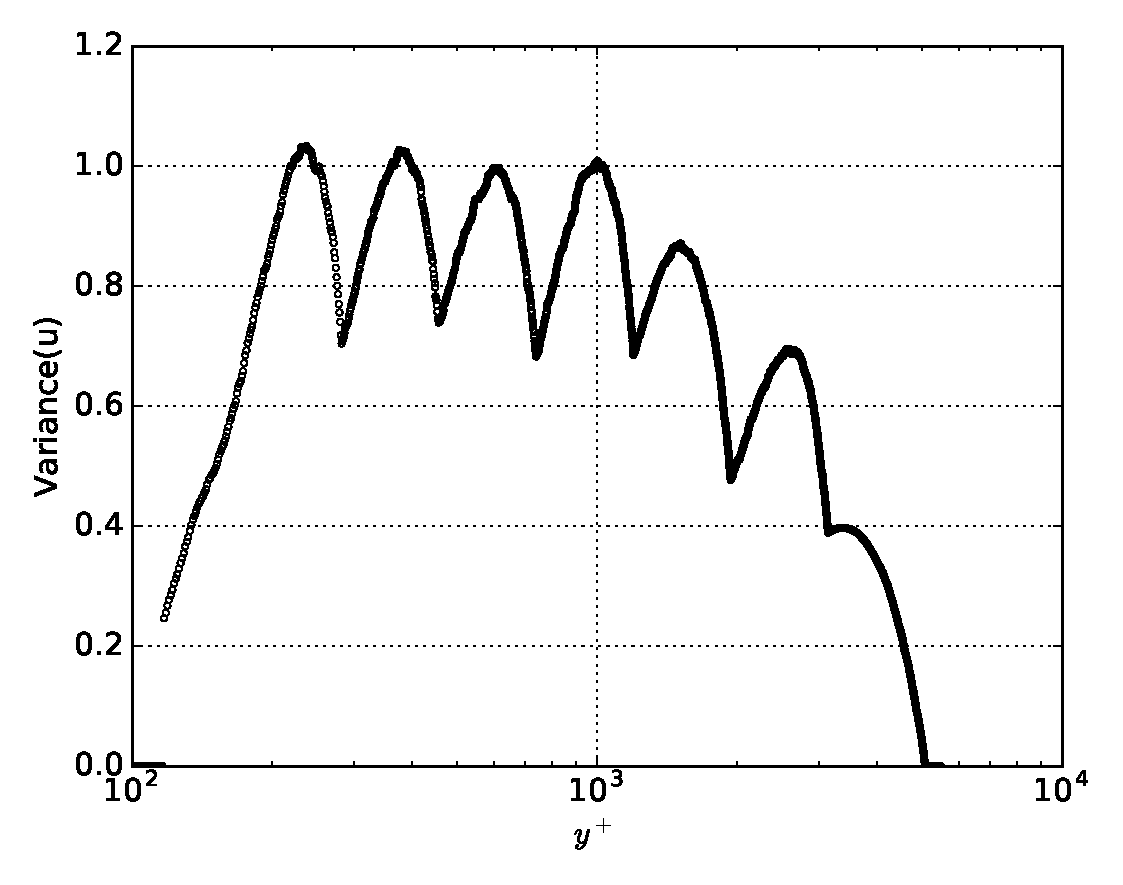
\includegraphics[scale=0.46]{figures/variance_5000_assembles_un130}
\caption{\label{fig:varun130} Variance of streamwise velocity fluctuations for 5000 independent realizations with an uniform perturbation of $\pm \%130$.}
\end{figure}     
The rapid variations still persist in the higher order moments, however their amplitude are smaller compared with the gaussian distribution for $\sigma=0.4$. Fig.~\ref{fig:skewun130} shows the skewness of the streamwise velocity for an uniform distribution. A strong agreement in the main features between the numerical simulation and the experimental skewness is observed, in brief the skewness follows a pseudo-Gaussian trend in the inertial region , then it increases up to reach its maximum negative value in the upper limit of the boundary layer $y^+=\delta^+$ to after finally decay to zero in the free-stream region.
\begin{figure}[tb]
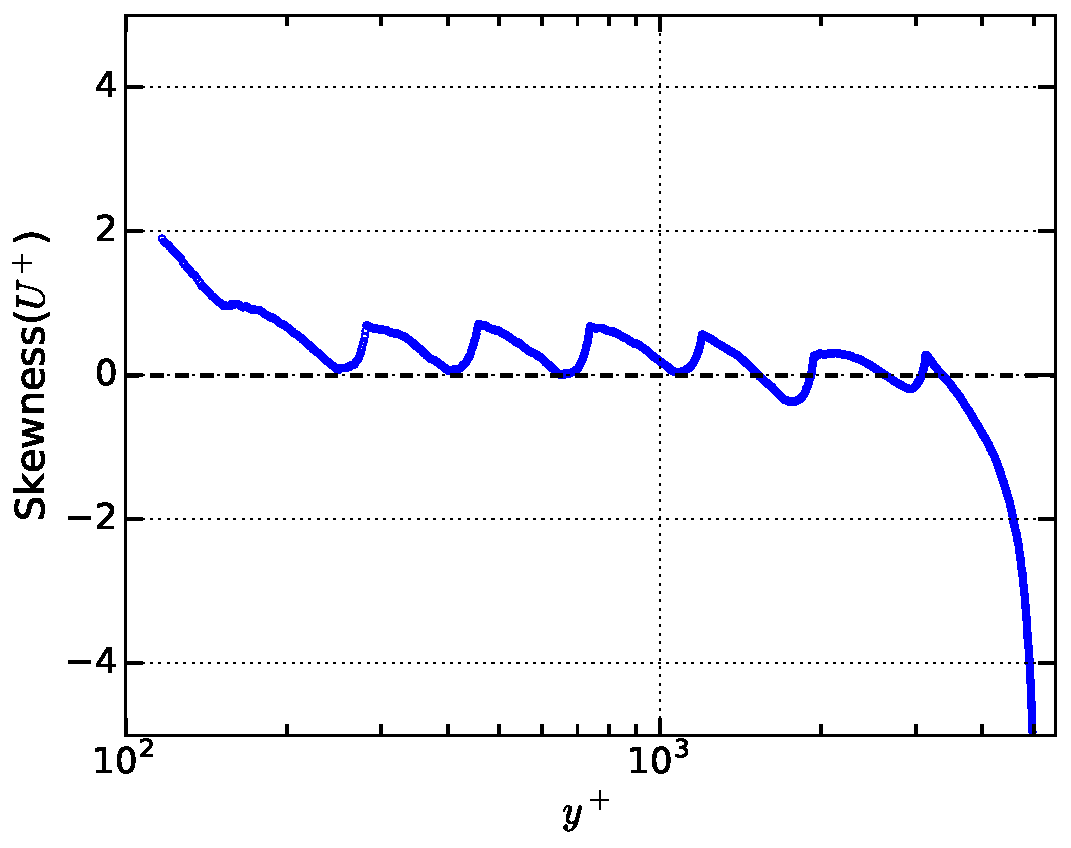
\includegraphics[scale=0.46]{figures/skewness_5000_assembles_un130}
\caption{\label{fig:skewun130} Skewness of streamwise velocity fluctuations for 5000 independent realizations with an uniform perturbation of $\pm 130\%$ (open circles). The skewness for a Gaussian distribution is plotted in dotted lines as a reference.}
\end{figure}
Fourth order moment is illustrated in Fig.~\ref{fig:kurtun130}, the trend is in complete concordance with the experimental data if the small oscillations are neglected. Further exploration is needed to improve the right behaviour in the upper and lower limits of the inertial region.
\begin{figure}[tb] 
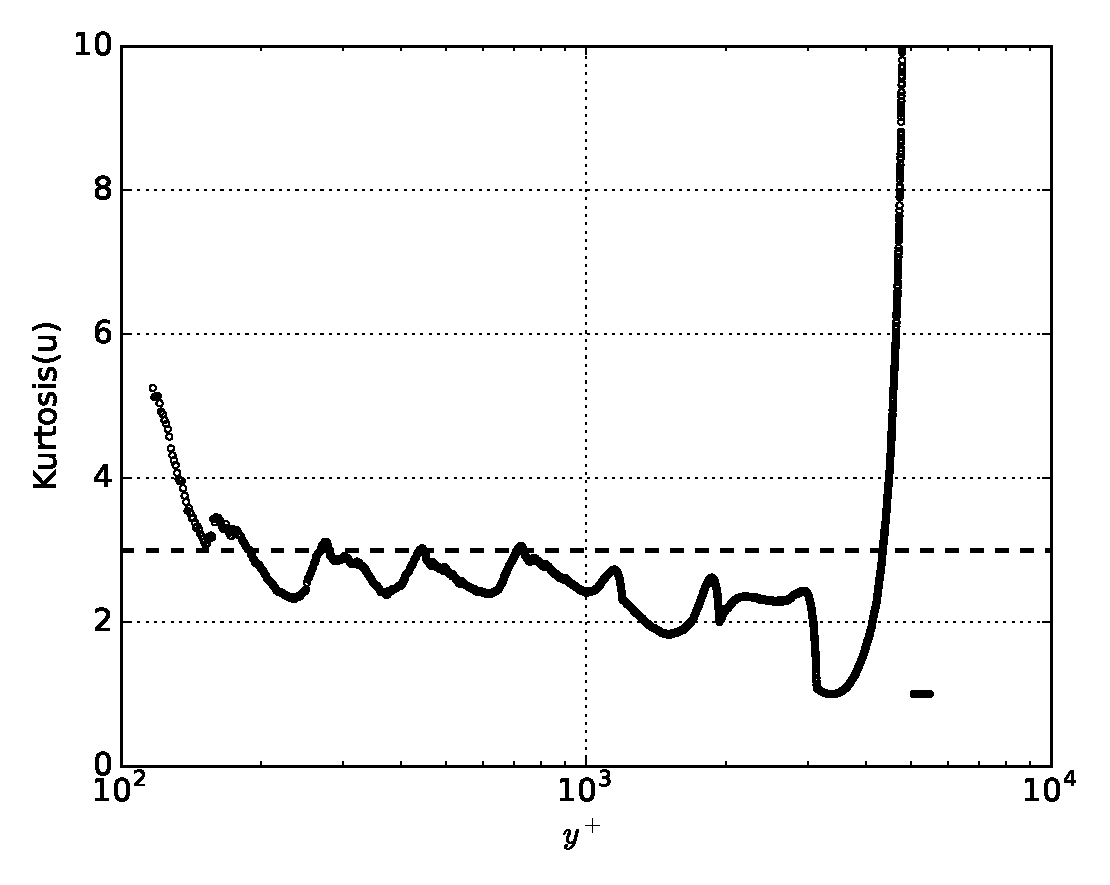
\includegraphics[scale=0.46]{figures/kurtosis_5000_assembles_un130}
\caption{\label{fig:kurtun130} Kurtosis of streamwise velocity fluctuations for 5000 independent realizations with an uniform perturbation of $\pm 130\%$ (open circles). The kurtosis for a Gaussian distribution is plotted in dotted lines as a reference.} 
\end{figure}


%\nocite{*}
\bibliography{Aps_template2}% Produces the bibliography via BibTeX.
\end{document}
